\documentclass{article}
\usepackage[12pt]{extsizes}
\usepackage[a4paper, margin=0.5cm]{geometry}
\usepackage{indentfirst}
\usepackage[T1, T2A]{fontenc}
\usepackage[english, russian]{babel}
\usepackage{amsmath, amssymb, fleqn, cancel, graphicx, wrapfig, tabbing, color, cases, lipsum}

\usepackage{amstext} % for \text macro
\usepackage{array}   % for \newcolumntype macro
\newcolumntype{L}{>{$}l<{$}} % math-mode version of "l" column type

\DeclareMathOperator{\rank}{rank}
\makeatletter
\newenvironment{sqcases}{%
  \matrix@check\sqcases\env@sqcases
}{%
  \endarray\right.%
}
\def\env@sqcases{%
  \let\@ifnextchar\new@ifnextchar
  \left\lbrack
  \def\arraystretch{1.2}%
  \array{@{}l@{\quad}l@{}}%
}
\makeatother

\DeclareRobustCommand{\divby}{\mathrel{\vbox{\baselineskip.65ex\lineskiplimit0pt\hbox{.}\hbox{.}\hbox{.}}}}

\setlength{\parindent}{0pt}

\newenvironment{rcases}
    {\left.\begin{aligned}}
    {\end{aligned}\right\rbrace}

\usepackage{hyperref}
\hypersetup{
    colorlinks,
    citecolor=black,
    filecolor=black,
    linkcolor=black,
    urlcolor=black
}




\begin{document}

\begin{titlepage}
    \title{Линейная алгебра и Аналитическая геометрия}
    \author{Бабицкий Иван | М8О-111БВ-24 \\ 02.03.02 "Фундаментальная информатика и информационные технологии"}
    \date{2024/2025 учебный год, 1-й семестр}
    \maketitle
    \begin{center}
        
\includegraphics[scale=0.2]{images/mai.png}
    \end{center}
\end{titlepage}

\tableofcontents




%--------------------------------------------------
\newpage
\paragraph{ЛК-1 | 2024.09.06 (1)}
\part{Матрицы и операции с ними}

\section{Введение}

\subsection{Определения | Матрица и её элементы}
\begin{itemize}
    \item Матрица $A$ порядка $m \times n$ ($m$ на $n$) --- это двумерная таблица чисел, состоящая из $m$ строк и $n$ столбцов.
    \item Каждый элемент матрицы A, лежащий на пересечении $i$-й строки и $j$-го столбца обозначается как $a_{ij}$.
\end{itemize}

\begin{gather*}
    A_{m \times n} \overset{\Delta}{=} \underset{i = \overline{1, m}, ~ j = \overline{1, n}}{\left( a_{ij} \right)} = \begin{vmatrix}
        a_{11} & a_{12} & \dots & a_{1n} \\
        a_{21} & a_{22} & \dots & a_{2n} \\
        \dots  & \dots  & \dots & \dots  \\
        a_{m1} & a_{m2} & \dots & a_{mn}
    \end{vmatrix}
\end{gather*}

\subsubsection{Примечание | Написание элементов}
...

\subsubsection{Примечание | Область определения элементов}
\[
    a_{ij} \in \mathbb{R} \text{ или } a_{ij} \in \mathbb{C}.
\]


\section{Виды матриц}




%--------------------------------------------------
\newpage
\paragraph{ЛК-8 | 2024.10.25 (1)}
~\\ \textbf{Аналитическая геометрия} --- изучение геометрический объектов с помощью математических моделей (уравнения, формулы).

\part{Алгебра векторов}

\section{Введение}

\subsection{Определение | Геометрический вектор}
Геометрическим вектором называется направленный отрезок прямой, который можно перемещать паралелльно себе.

\subsubsection{Виды векторов}
\begin{itemize}
    \item Свободный
    \item Фиксированный
\end{itemize}

\includegraphics[scale=0.2]{images/2024-10-25/01.jpg}


\subsection{Определение | Модуль вектора}
Модулем вектора $\overline{a}$ называется число, определяющее его длину: $|\overline{a}| \in \mathbb{R}$


\subsection{Определение | Нулевой вектор}
Нулевым вектором $\overline{0}$ называется вектор с нулевой длиной (начало и конец совпадают).
\[
|\overline{0}| = 0,  \overline{0} = \overline{AA}
\]


\subsection{Определение | Коллинеарные векторы}
Коллинеарными называют 2 и более векторов, которые параллельны одной и той же прямой.
\[
    \overline{a}, \overline{b}, \overline{c}, \dots \Rightarrow 
    \overline{a} \parallel \overline{b} \parallel \overline{c} \parallel \dots
\]
\begin{align*}
    \overline{a} \parallel \overline{b} =
    \begin{sqcases}
        \overline{a} \uparrow \uparrow \overline{b} \text{ --- сонаправленные} \\
        \overline{a} \uparrow \downarrow \overline{b} \text{ --- противонаправленные} \\
    \end{sqcases}
\end{align*}

\includegraphics[scale=0.3]{images/2024-10-25/02.jpg}


\subsection{Определение | Компланарные векторы}
Компланарными называются 3 и более векторов в пространстве, которые параллельны одной и той же плоскости:
\[
    (\overline{a}, \overline{b}, \overline{c}, \dots) \parallel P
\]

\includegraphics[scale=0.15]{images/2024-10-25/03.jpg}



\par\noindent\rule{\textwidth}{1pt}
\section{Линейные операции над векторами}

\subsection{Равенство}
\begin{gather*}
    \overline{a} = \overline{b} \Leftrightarrow
    \begin{cases}
        \overline{a} \upuparrows \overline{b} \\
        |\overline{a}| = |\overline{b}|
    \end{cases}
\end{gather*}


\subsection{Сложение}

\subsubsection{Если компланарны}
Правила параллелограмма и треугольника соответственно: \\

\includegraphics[scale=0.15]{images/2024-10-25/04.jpg}

\subsubsection{Если некомпланарны}
Сумма --- диагональ паралеллограмма: \\

\includegraphics[scale=0.2]{images/2024-10-25/05.jpg}

\subsubsection{Способы}
\begin{itemize}
    \item $\overline{a} + \overline{b} = \overline{b} + \overline{a}$
    \item $(\overline{a} + \overline{b}) + \overline{c} = \overline{a} + (\overline{b} + \overline{c})$
    \item $\overline{a}_1 + \overline{a}_2 + \overline{a}_3 + \overline{a}_4 = \overline{e}$
\end{itemize}

\includegraphics[scale=0.2]{images/2024-10-25/06.jpg}


\subsection{Умножение на число $\lambda \in \mathbb{R}$}
\begin{gather*}
    \lambda \overline{a} \overset{\Delta}{=} \overline{b}:
    \begin{cases}
        \overline{b} \upuparrows \overline{a}, \text{ если } \lambda > 0 \\
        \overline{b} \uparrow \downarrow  \overline{a}, \text{ если } \lambda < 0 \\
        |\overline{b}| = |\lambda||\overline{a}|
    \end{cases}
\end{gather*}

\includegraphics[scale=0.3]{images/2024-10-25/07.jpg}

\subsubsection{Противоположный вектор}
\[
    \overline{b} = (-1)\overline{a} = -\overline{a}
\]

\subsubsection{Единичный вектор направления $\overline{a}$}
\begin{gather*}
    \overline{a}^0 \overset{\Delta}{=} \frac{\overline{a}}{|\overline{a}|} ~\Rightarrow~
    |\overline{a}^0| = \frac{|\overline{a}|}{|\overline{a}|} = 1 ~~~~~
    \begin{cases}
        \overline{a}^0 \upuparrows \overline{a} \\
        |\overline{a}|^0 = 1
    \end{cases}
\end{gather*}


\par\noindent\rule{\textwidth}{1pt}
\section{Свойства коллинеарных векторов}

\subsection{Всегда пропорциональны}
\[
    \overline{a} \parallel \overline{b} \Rightarrow \exists \lambda \in \mathbb{R}: \overline{b} = \lambda \overline{a}
\]



\section{Системы координат на плоскости и в пространстве}

\subsection{Афинные}

\subsubsection{Прямоугольная декартова}
\textit{(изображение)}


\subsection{Не афинные}

\subsubsection{Полярная}
\textit{(изображение)}

\subsubsection{Цилиндрическая}
\textit{(изображение)}

\subsubsection{Сферическая}
\textit{(изображение)}

\subsection{Общие афинные}

\subsubsection{Косоугольная}
\textit{(изображение)}
\subsubsection{Не декартова}
\textit{(изображение)}

\subsection{Определение | Базис на плоскости}
Базисом на плоскости называется любая пара неколлениарных векторов, лежащих на этой плоскости. 
~~~~~ $\{\overline{e}_1, \overline{e}_2\}$ \\

\includegraphics[scale=0.2]{images/2024-10-25/08.jpg}

\subsubsection{Свойства}
Любой третий вектор $\overline{a} \in P$ (линейно-зависимый) может быть представлен в виде линейной комбинации векторов базиса.

\section{Выражение $\overline{a} \cdot \overline{b}$ через декартовы координаты $\overline{a}$ и $\overline{b}$}
\begin{gather*}
    \text{Пусть } \overline{a} = a_x \overline{i} + a_y \overline{j} + a_z \overline{k} = 
    (a_x, a_y, a_z)_{(\overline{i}, \overline{j}, \overline{k})} \\
    \overline{b} = b_x \overline{i} + b_y \overline{j} + b_z \overline{k} = 
    (b_x, b_y, b_z)_{(\overline{i}, \overline{j}, \overline{k})} \\
    \text{Тогда } \overline{a} \cdot \overline{b} =
    (a_x \overline{i} + a_y \overline{j} + a_z \overline{k}) \cdot (b_x \overline{i} + b_y \overline{j} + b_z \overline{k}) = \\
    a_x(b_x \underbrace{\overline{i} \cdot \overline{i}}_{1} + b_y \underbrace{\overline{i} \cdot \overline{j}}_{0} + b_z \underbrace{\overline{i} \cdot \overline{k}}_{0}) +
    a_y(b_x \underbrace{\overline{j} \cdot \overline{i}}_{0} + b_y \underbrace{\overline{j} \cdot \overline{j}}_{1} + b_z \underbrace{\overline{j} \cdot \overline{k}}_{0}) +
    a_z(b_x \underbrace{\overline{k} \cdot \overline{i}}_{0} + b_y \underbrace{\overline{k} \cdot \overline{j}}_{0} + b_z \underbrace{\overline{k} \cdot \overline{k}}_{1}) \\
    \text{Итого: } \overline{a} \cdot \overline{b} = (\overline{a_x, a_y, a_z}) \cdot (\overline{b_x, b_y, b_z}) =
    a_x b_x + a_y b_y + a_z b_z
\end{gather*}



\section{Произведения геометрических векторов}

\subsection{Скалярное}

\subsubsection{Определение}
\begin{gather*}
    \text{Число } = (\overline{a}, \overline{b}) \equiv \overline{a} \cdot \overline{b} \overset{\Delta}{=}
    |\overline{a}| \cdot \underbrace{|\overline{b}| \cdot \cos \varphi}_{\text{Пр}_{\overline{a}} \overline{b}}
    ~~~~~ \varphi = \widehat{\overline{a}, \overline{b}} \in \left[ 0; \pi \right] 
\end{gather*}


\subsubsection{Геометрический смысл}
(рисунок)


\subsubsection{Вычисление}
\begin{align*}
    \begin{rcases}
        \overline{a} = a_x \overline{i} + a_y \overline{j} + a_z \overline{k} = \{a_x, a_y, a_z\} \\
        \overline{b} = b_x \overline{i} + b_y \overline{j} + b_z \overline{k} = \{b_x, b_y, b_z\}
    \end{rcases} \Rightarrow
    \overline{a} \cdot \overline{b} = \boxed{a_x b_x + a_y b_y + a_z b_z}
\end{align*}


\subsubsection{Свойства}

\paragraph{???}
\[
    \text{Пр}_{\overline{a}} \overline{b} = |\overline{b}| \cdot \cos \varphi \Rightarrow
    \overline{a} \cdot \overline{b} = |\overline{a}| \cdot  \text{Пр}_{\overline{a}} \overline{b}
\]
\[
    \text{Пр}_{\overline{a}} \overline{b} = \frac{\overline{a} \cdot \overline{b}}{|\overline{a}|}
\]

\paragraph{Равенство нулю}
\begin{align*}
    \overline{a} \cdot \overline{b} = 0 \Leftrightarrow
    \begin{sqcases}
        \overline{a} \bot \overline{b}, \text{ так как } \cos \varphi = 0 \\
        \overline{a} = \overline{0} \text{ или } \overline{b} = \overline{0}
    \end{sqcases}
\end{align*}

\paragraph{???}
\[
    (\overline{a} + \overline{b}, \overline{c}) = 
    (\overline{a} + \overline{b}) \cdot \overline{c} =
    \overline{a} \cdot \overline{c} + \overline{b} \cdot \overline{c}
\]

\paragraph{???}
\begin{gather*}
    (\lambda \overline{a}) \cdot \overline{b} = \lambda(\overline{a} \cdot \overline{b}) \\
    (\lambda \overline{a}, \overline{b}) = \lambda(\overline{a}, \overline{b})
\end{gather*}


\paragraph{Линейность}
\[
    (\alpha \overline{a} + \beta \overline{b}) \cdot \overline{c} =
    \alpha (\overline{a} \cdot \overline{c}) + \beta (\overline{b} \cdot \overline{c})
\]

\paragraph{???}
\[
    \overline{a} \cdot \overline{a} = |\overline{a}||\overline{a}| \cdot \cos 0 = |\overline{a}|^2
\]

\paragraph{Коммутативность}
\[
    \overline{a} \cdot \overline{b} = \overline{b} \cdot \overline{a}
\]

\paragraph{???}
\[
    \overline{a} \cdot \overline{b} = |\overline{a}| \cdot \text{Пр}_{\overline{a}} \overline{b}
\]


\subsubsection{Применение}

\paragraph{???}
\[
    |\overline{a}| = \sqrt{\overline{a} \cdot \overline{a}} = \sqrt{a_x^2 + a_y^2 + a_z^2}
\]

\paragraph{???}
\[
    \cos \varphi = \frac{\overline{a} \cdot \overline{b}}{|\overline{a}| \cdot |\overline{b}|}
\]


\par\noindent\rule{\textwidth}{1pt}
\subsection{Векторное}

\subsubsection{Определение}
\[
    \text{Вектор } = \left[ \overline{a}, \overline{b} \right] \equiv \overline{a} \times \overline{b} = \overline{n}:
\]
\begin{itemize}
    \item $\overline{n} \bot \overline{a}, \overline{n} \bot \overline{b}$
    \item Тройка $\overline{a}, \overline{b}, \overline{n}$ --- правая ($\overline{n}$ --- по правилу буравчика)
    \item $|\overline{n}| = |\overline{a}| \cdot |\overline{b}| \cdot \sin \varphi = S_{\#}$
\end{itemize}


\subsubsection{Геометрический смысл}
(рисунок)

\subsubsection{Вычисление (через декартовы прямые координаты)}
\begin{gather*}
    \overline{n} = \overline{a} \times \overline{b} =
    \begin{vmatrix}
        \overline{i} & \overline{j} & \overline{k} \\
        a_x          & a_y          & a_z          \\
        b_x          & b_y          & b_z
    \end{vmatrix} =
    A_{11} \overline{i} + A_{12} \overline{j} + A_{13} \overline{k} =
    \{\underbrace{A_{11}}_{n_x}, \underbrace{A_{12}}_{n_y}, \underbrace{A_{13}}_{n_z}\}
\end{gather*}


\subsubsection{Свойства}

\paragraph{???}
\[
    \overline{a} \times \overline{b} = -\overline{b} \times \overline{a}
\]

\paragraph{???}
\begin{align*} 
    \begin{rcases}
        \overline{a} \times \overline{b} = \overline{0} \\
        \overline{a} \neq \overline{0}, \overline{b} \neq \overline{0}    
    \end{rcases} \Leftrightarrow 
    \overline{a} \parallel \overline{b} 
\end{align*}

\paragraph{???}
\[
    \overline{a} \times \overline{a} = \overline{0}
\]

\paragraph{???}
\[
    \left( \alpha_1 \overline{a}_1 + \alpha_2 \overline{a}_2 \right) \times \overline{b} =
    \alpha_1 \underbrace{\overline{a}_1 \times \overline{b}}_{\neq \overline{b} \times \overline{a}_1} +
    \alpha_2 \overline{a}_2 \times \overline{b}
\]


\subsubsection{Применение}

\paragraph{Площадь паралеллограмма}
\[
    S_{\#}^{\overline{a}, \overline{b}} = \left| \overline{a} \times \overline{b} \right|
\]

\paragraph{Направление нормали}
\[
    \overline{n} = \overline{a} \times \overline{b} \text{ --- нормаль к плоскости } P \parallel \overline{a}, \overline{b}
\]


\par\noindent\rule{\textwidth}{1pt}
\subsection{Смешанное (векторно-скалярное)}

\subsubsection{Определение}
\begin{gather*}
    \text{Число } = (\overline{a}, \overline{b}, \overline{c}) \overset{\Delta}{=}
    (\overbrace{\overline{a} \underbrace{\times}_{(1)} \overline{b}}^{\overline{n}}) \underbrace{\cdot}_{(2)} \overline{c}
\end{gather*}

\subsubsection{Геометрический смысл}
(рисунок)

\subsubsection{Вычисление}
\begin{gather*}
    (\overline{a}, \overline{b}, \overline{c}) =
    \begin{vmatrix}
        a_x & a_y & a_z \\
        b_x & b_y & b_z \\
        c_x & c_y & c_z
    \end{vmatrix}
\end{gather*}
\paragraph{Проверка по $\overline{n} = \overline{a} \times \overline{b}$}
\[
    \overline{n} \cdot \overline{c} \overset{?}{=} (\overline{a}, \overline{b}, \overline{c})
\]


\subsubsection{Свойства}

\paragraph{Перестановки круговые}
\[
    (\overline{a}, \overline{b}, \overline{c}) =
    (\overline{b}, \overline{c}, \overline{a}) =
    (\overline{c}, \overline{a}, \overline{b}) =
    (\overline{a}, \overline{b}, \overline{c})
\]

\paragraph{Перестановки соседей}
\[
     (\overline{a}, \overline{b}, \overline{c}) =
    -(\overline{b}, \overline{a}, \overline{c})
\]
\[
     (\overline{a}, \overline{b}, \overline{c}) =
    -(\overline{a}, \overline{c}, \overline{b})
\]

\paragraph{???}
\[
    \left( \left( \alpha_1 \overline{a}_1 + \alpha_2 \overline{a}_2 \right), \overline{b}, \overline{c} \right) =
    \alpha_1 \left( \overline{a}_1, \overline{b}, \overline{c} \right) +
    \alpha_2 \left( \overline{a}_2, \overline{b}, \overline{c} \right)
\]

\paragraph{Компланарная тройка}
\begin{align*}
    \begin{rcases}
        (\overline{a}, \overline{b}, \overline{c}) = 0 \\
        \overline{a} \neq \overline{0}, \overline{b} \neq \overline{0}, \overline{c} \neq \overline{0} 
    \end{rcases} \Leftrightarrow
    \overline{a}, \overline{b}, \overline{c} \text{ --- тройка компланарна}
\end{align*}


\subsubsection{Применение}

\paragraph{Объём параллелепипеда}
\[
    V_{\#}^{\overline{a}, \overline{b}, \overline{c}} = \left| \left( \overline{a}, \overline{b}, \overline{c} \right) \right|
\]

\paragraph{Знак}
\begin{itemize}
    \item $\left( \overline{a}, \overline{b}, \overline{c} \right) > 0 \Leftrightarrow$ тройка правая
    \item $\left( \overline{a}, \overline{b}, \overline{c} \right) < 0 \Leftrightarrow$ тройка левая
\end{itemize}



\newpage
\paragraph{ЛК-9 | 2024.11.15 (1)}

\section{Взаимное расположение прямых на плоскости}
\paragraph{Дано}
\begin{gather*}
    l_1: A_1x + B_1y + C_1 = 0 \Rightarrow \overline{N}_1 = \{A_1, B_1\} \bot l_1
    l_2: A_2x + B_2y + C_2 = 0 \Rightarrow \overline{N}_2 = \{A_2, B_2\} \bot l_2
\end{gather*}

\subsection{Случай 1}
\begin{gather*}
    l_1 \parallel l_2 \Leftrightarrow \overline{N}_1 \parallel \overline{N_2} \Leftrightarrow \exists t \in \mathcal{R}: \overline{N}_1 = t\overline{N}_2 \\
    \{A_1 B_1\} = t\{A_2, B_2\} \\
    \begin{cases}
        A_1 = tA_2 \\
        B_1 = tB_2
    \end{cases} \\
    t = \frac{A_1}{A_2} = \frac{B_1}{B_2}
\end{gather*}

\section{Расстояние между паралелльными прямыми}
\begin{gather*}
    \rho(l_1 \parallel l_2) \overset{\Delta}{=} \rho(M_1 \in l_1, l_2) = \text{ смотреть выше} \\
    M_1 = (x_1, y_1) \in l_1: A_1x_1 + B_1y_1 + C_1 = 0
\end{gather*}





%--------------------------------------------------
\newpage
\paragraph{ЛК-10 | 2024.11.15 (1)}
\part{Плоскость $P$ в пространстве $Oxyz$}

\section{Общее уравнение плоскости $P$}
\begin{gather*}
    \begin{cases}
        M_0(x_0, y_0, z_0) \in P \\
        \overline{N}\{A, B, C\} \bot P
    \end{cases} \Rightarrow
    \forall M(x, y, z) \in P: \overline{M_0 M} \bot \overline{N} \\
    \overline{N} \cdot \overline{M_0 M} = 0 \\
    \{A, B, C\} \cdot \{x - x_0, y - y_0, z - z_0\} = 0 \\
    \boxed{A(x - x_0) + B(y - y_0) + C(z - z_0) = 0} \Rightarrow \\
    \Rightarrow \boxed{Ax + By + Cz + D = 0}, \text{ где } D = - Ax_0 - By_0 - Cz_0 \\
    \{A, B, C\} \bot P ~~~ |D| \sim \rho(O, P)
\end{gather*}

\includegraphics[scale=0.3]{images/2024-11-15/01.png}



\section{Параметрические и компланарные уравнения плоскости}
\paragraph{Дано}
\begin{gather*}
    \begin{cases}
        M_0(x_0, y_0, z_0) \in P \\
        \overline{p} = \{p_x, p_y, p_z\} \parallel P \\
        \overline{q} = \{q_x, q_y, q_x\} \parallel P \\
        \overline{p} \nparallel \overline{q}
    \end{cases} \Rightarrow
\end{gather*}

\includegraphics[scale=0.3]{images/2024-11-15/02.png}

\subsection{Случай 1}
\begin{gather*}
    \Rightarrow \forall M(x, y, z) \in P: \overline{M_0M}, \overline{p}, \overline{q} \text{ --- компланарны} \\
    (\overline{M_0M}, \overline{p}, \overline{q}) = 0 \\
    \begin{vmatrix}
        x - x_0 & y - y_0 & z - z_0 \\
        p_x     & p_y     & p_z     \\
        q_x     & q_y     & q_x
    \end{vmatrix} = 0 \\
    \underset{\text{общее уравнение}}{\boxed{(x - x_0)A_{11} + (y - y_0)A_{12} + (z - z_0)A_{13} = 0}}  
\end{gather*}


\subsection{Случай 2}
\begin{gather*}
    \exists t_1, t_2 \in \mathbb{R}: \overline{M_0M} = t_1 \overline{p} + t_2 \overline{q} \\
    \begin{cases}
        x - x_0 = t_1 p_x + t_2 q_x \\
        y - y_0 = t_1 p_y + t_2 q_y \\
        z - z_0 = t_1 p_z + t_2 q_z
    \end{cases}
\end{gather*}

\includegraphics[scale=0.3]{images/2024-11-15/03.png}



\section{Уравнение плоскости через 3 точки, не лежащие на одной прямой}
\paragraph{Дано}
\begin{gather*}
    \begin{cases}
        M_1 \in P \\
        N_2 \in P \\
        M_3 \in P \\
        \overline{M_1 M_2} \nparallel \overline{M_1 M_3}
    \end{cases} \Rightarrow
    \begin{cases}
        M_0 = M_1 \\
        \overline{p} = \overline{M_1 M_2} \\
        \overline{q} = \overline{M_1 M_3} \\
        \overline{p} \nparallel \overline{q} 
    \end{cases} \\
    P: \begin{vmatrix}
        x   - x_1 & y   - y_1 & z   - z_1 \\
        x_2 - x_1 & y_2 - y_1 & z_2 - z_1 \\
        x_3 - x_1 & y_3 - y_1 & z_3 - z_1 \\
    \end{vmatrix} = 0 \rightarrow
    Ax + By + Cz + D = 0
\end{gather*}

\includegraphics[scale=0.3]{images/2024-11-15/04.png}



\section{Уравнение плоскости в отрезках}

\includegraphics[scale=0.3]{images/2024-11-15/05.png}
\begin{gather*}
    \Rightarrow \begin{vmatrix}
        x - a & y - 0 & z - 0 \\
        0 - a & b - 0 & 0 - 0 \\
        0 - a & 0 - 0 & c - 0
    \end{vmatrix} = 0 \\
    \frac{x}{a} + \frac{y}{b} + \frac{z}{c} = 1
\end{gather*}



\section{Расстояние от точки $M_1$ до $P$}
\[
    Ax + By + Cz + D = 0
\]

\includegraphics[scale=0.3]{images/2024-11-15/06.png}
\paragraph{Дано}
\begin{gather*}
    \begin{cases}
        M_1(x_1, y_1, z_1) \\
        P: Ax + By + Cz + D = 0
    \end{cases} \Rightarrow
    \rho(M_1, P) \text{ --- ?}
\end{gather*}
\paragraph{Решение}
\begin{gather*}
    \overline{N} = \{A, B, C\} \bot P \\
    \text{Пусть } M_0 \in P: \\
    Ax_0 + By_0 + Cz_0 + D = 0 \\
    \rho(M_1, P) = \underbrace{M_1 k}_{\ge 0} = 
    \left| \underbrace{\text{Пр}_{\overline{N}} \overline{M_0 M_1}}_{\gtrless 0} \right| = 
    \left| \frac{\overline{N} \cdot \overline{M_0 M_1}}{\left| \overline{N} \right|} \right| = \\
    = \frac{\left| A(x_1 - x_0) + B(y_1 - y_0) + C(z_1 - z_0) \right|}{\left| \overline{N} \right|} =
    \frac{\left| Ax_1 + By_1 + Cz_1 + (\overbrace{-Ax_0 - By_0 - Cz_0}^{= D}) \right|}{\left| \overline{N} \right|} \\
    \rho(M_1(x_1, y_1, z_1); P: Ax + By + Cz + D = 0) = 
    \frac{\left| Ax_1 + By_1 + Cz_1 + D \right|}{\sqrt{A^2 + B^2 + C^2}}
\end{gather*}


\subsection{Геометрический смысл $D$}
\begin{gather*}
    \rho(O(0, 0, 0); P: Ax + By + Cz + D = 0) = 
    \frac{\left| A \cdot 0 + B \cdot 0 + C \cdot 0 + D \right|}{\left| \overline{N} \right|}
\end{gather*}


\subsection{Следствие}
\[
    \left| D \right| = \rho(O, P) \cdot \left| \overline{N} \right|
\]



\section{Взаимное расположение $P_1$ и $P_2$ в $Oxyz$}
\paragraph{Дано}
\begin{gather*}
    P_1: A_1x + B_1y + C_1z + D_1 = 0 \Rightarrow \overline{N_1} = \{A_1, B_1, C_1\} \bot P_1 \\
    P_2: A_2x + B_2y + C_2z + D_2 = 0 \Rightarrow \overline{N_2} = \{A_2, B_2, C_2\} \bot P_2 
\end{gather*}

\subsection{Случай 1}
\begin{gather*}
    P_1 \parallel P_2 \Leftrightarrow 
    \overline{N_1} \parallel \overline{N_2} \Leftrightarrow
    \exists t \in \mathbb{R}: \overline{N_1} = t \overline{N_2} \\
    t = \frac{A_1}{A_2} = \frac{B_1}{B_2} = \frac{C_1}{C_2}
\end{gather*}

\includegraphics[scale=0.3]{images/2024-11-15/07.png}

\paragraph{Характеристика $P_1 \parallel P_2$ --- расстояние между ними}
\begin{gather*}
    \rho(P \parallel P) \overset{\Delta}{=} \rho(M_1 \in P_1, P_2) = 
    \frac{\left| A_2 x_1 + B_2 y_1 + C_2 z_1 + D_2 \right|}{\sqrt{A^2_2 + B^2_2 + C^2_2}}
\end{gather*}

\includegraphics[scale=0.3]{images/2024-11-15/08.png}


\subsection{Случай 2}
\begin{gather*}
    P_1 \nparallel P_2 \Leftrightarrow
    \text{ или } \frac{A_1}{A_2} \neq \frac{B_1}{B_2}, \text{ или } \frac{B_1}{B_2} \neq \frac{C_1}{C_2}
\end{gather*}


\subsubsection{Линия пересечения}

\includegraphics[scale=0.3]{images/2024-11-15/09.png}
\begin{gather*}
    L = P_1 \cap P_2 \\
    L: \underset{\text{Общие уравнения } L \in Oxyz}{
        \boxed{\begin{cases}
        A_1 x + B_1 y + C_1 z + D_1 = 0 \\
        A_2 x + B_2 y + C_2 z + D_2 = 0
    \end{cases}}}
\end{gather*}
\paragraph{Об уравнениях:}
\begin{itemize}
    \item $\exists$ одно паралелльное множество решений $M(x, y, z) \in L$
    \item Они линейно независимые
\end{itemize}

\subsubsection{Угол между плоскостями}

\includegraphics[scale=0.3]{images/2024-11-15/10.png}
\begin{gather*}
    \alpha = \widehat{P_1, P_2} \in \left[ 0 ; \frac{\pi}{2} \right] \text{ --- острый} ~~~~~
    \varphi = \widehat{\overline{N_1}, \overline{N_2}} \in \left[ 0 ; \pi \right] ~~~~~
    \alpha + \varphi = \pi \\
    \underbrace{\cos \alpha}_{\ge 0} =
    \left| \underbrace{\cos \varphi}_{\lessgtr 0} \right| =
    \frac{\left| \overline{N_1} \cdot \overline{N_2}\right|}{\left| \overline{N_1} \right| \cdot \left| \overline{N_2} \right|} =
    \frac{\left| A_1 A_2 + B_1 B_2 + C_1 C_2 \right|}{\sqrt{A_1^2 + B_1^2 + C_1^2} + \sqrt{A_2^2 + B_2^2 + C_2^2}}
\end{gather*}




%--------------------------------------------------
\newpage
\paragraph{ЛК-11 | 2024.11.22}
\part{Прямая линия $L$ в пространстве $Oxyz$}

\section{Основные уравнения прямой линии}

\includegraphics[scale=0.3]{images/2024-11-22/01.png}
\begin{gather*}
    L = P_1 \overbrace{\cap}^{\exists} P_2 \Rightarrow M(x, y, z) \in L \\
    \boxed{L: \begin{cases}
        A_1x + B_1y + C_1z + D_1 = 0 ~~~ (M \in P_1) \\
        A_2x + B_2y + C_2z + D_2 = 0 ~~~ (M \in P_2) \\
    \end{cases}} ~~~ (\text{ЛНЗ уравнения}) \\
    \exists L: \frac{A_1}{A_2} \neq \frac{B_1}{B_2} \text{ или } \frac{B_1}{B_2} \neq \frac{C_1}{C_2}
\end{gather*}


\section{Параметрические и канонические уравнения прямой линии $L$}

\includegraphics[scale=0.2]{images/2024-11-22/02.png}
\begin{align*}
    \begin{rcases}
        M_0(x_0, y_0, z_0) \in L \\
        \overline{q} =\{m, n, p\} \parallel L
    \end{rcases} \Rightarrow
    \forall M(x, y, z) \in L ~~~~~ \overline{M_0 M} \parallel \overline{q}
\end{align*}
\begin{gather*}
    \exists t \in \mathbb{R}: \overline{M_0 M} = t \overline{q} \Leftrightarrow
    \begin{cases}
        x - x_0 = tm \\
        y - y_0 = tn \\
        z - z_0 = tp
    \end{cases} \\
    \boxed{t = \frac{x - x_0}{m} = \frac{y - y_0}{n} = \frac{z - z_0}{p}} \\
    \overline{q} \neq \overline{0}: \boxed{m^2 + n^2 + p^2 \neq 0}
\end{gather*}

\subsection{Пример}

\includegraphics[scale=0.3]{images/2024-11-22/03.png}
\begin{gather*}
    \frac{x - 1}{0} = \frac{y - 2}{0} = \frac{z + 3}{4} \Rightarrow
    \overline{q} = \{0; 0; 4\} \parallel Oz \\
    \underbrace{x = 1}_{P_1 \bot Ox}, \underbrace{y = 2}_{P_2 \bot Oy}, z \in \mathbb{R} ~~~ 
    \overline{N_1} = \{1; 0; 0\} \bot P
\end{gather*}



\section{Уравнение прямой линии $L$ через 2 точки}

\includegraphics[scale=0.3]{images/2024-11-22/04.png}
\begin{align*}
    \begin{rcases}
        M_1(x_1, y_1, z_1) \in L \\
        M_2(x_2, y_2, z_2) \in L
    \end{rcases} \Rightarrow
    \boxed{\frac{x - x_1}{x_2 - x_1} = \frac{y - y_1}{y_2 - y_1} = \frac{z - z_1}{z_2 - z_1}}
\end{align*}


\section{Уравнение прямой линии $L$ в проекциях на координаты плоскости}
\begin{gather*}
    L: \frac{x - x_0}{m} = \frac{y- y_0}{n} = \frac{z - z_0}{p} \\
    \underbrace{\frac{x - x_0}{m} = \frac{y - y_0}{n}}_{\text{ЛНЗ}} \text{ --- уравнение } P_1 \parallel Oz \text{ и уравнение } \underbrace{l_{xy}}_{\text{Пр}_{Oxy} L} \in Oxy \\
    \underbrace{\frac{y - y_0}{n} = \frac{z - z_0}{p}}_{\text{ЛНЗ}} \text{ --- уравнение } P_2 \parallel Ox \text{ и уравнение } \underbrace{l_{yz}}_{\text{Пр}_{Oyz} L} \in Oyz \\
    \underbrace{\frac{x - x_0}{n} = \frac{z - z_0}{p}}_{\text{ЛЗ} } \text{ --- уравнение } P_3 \parallel Oy \text{ и уравнение } \underbrace{l_{xz}}_{\text{Пр}_{Oxz} L} \in Oxz \\
\end{gather*}

\includegraphics[scale=0.3]{images/2024-11-22/05.png}


\section{Расстояние от точки до прямой линии $L$}

\includegraphics[scale=0.3]{images/2024-11-22/06.png}
\begin{gather*}
    L: \frac{x - x_0}{m} = \frac{y- y_0}{n} = \frac{z - z_0}{p} \\
    \text{Из числителей: }   M_0(x_y, y_0, z_o) \in L \\
    \text{Из знаменателей: } \overline{q} = \{m, n, p\} \parallel L \\
    \rho (M_1, L) = h_{\#}^{\overline{M_0 M}, \overline{q}} = 
    \frac{S_{\#}^{\overline{M_0 M_1}, \overline{q}}}{\left| \overline{q} \right|} =
    \frac{\left| \overline{M_0 M_1} \times \overline{q} \right|}{\left| \overline{q} \right|}
\end{gather*}



\section{Взаимное расположение прямой линии $L$ и плоскости $P$}
\paragraph{Дано}
\begin{gather*}
    L: \frac{x - x_0}{m} = \frac{y- y_0}{n} = \frac{z - z_0}{p} \\
    \text{Из числителей: }   M_0(x_y, y_0, z_o) \in L \\
    \text{Из знаменателей: } \overline{q} = \{m, n, p\} \parallel L \\
    P: Ax + By + Cz + D = 0 \rightarrow \overline{N} = \{A, B, C\} \bot P
\end{gather*}

\subsection{Случай 1}
\[
    L \parallel P \Rightarrow \overline{N} \bot \overline{q}
\]
\begin{gather*} 
    \overline{N} \cdot \overline{q} = 0 \\
    \boxed{Am + Bn + Cp = 0} \text{ --- условие паралелльности}
\end{gather*}

\includegraphics[scale=0.3]{images/2024-11-22/07.png}

\subsubsection{Характеристика}
\begin{gather*}
    \rho(L \parallel P) = \rho(M_0 \in L, P) = 
    \frac{\left| Ax_0 + By_0 + Cz_0 + D \right|}{\sqrt{A^2 + B^2 + C^2}} \\
    \rho = 0 \Rightarrow L \subset P, ~~~ \rho \neq 0 \Rightarrow L \subset P, L = L_1
\end{gather*}


\subsection{Случай 2}
\[
    L \nparallel P \Rightarrow \boxed{Am + Bn + Cp \neq 0}
\]

\includegraphics[scale=0.3]{images/2024-11-22/08.png}

\subsubsection{Характеристики}
\paragraph{Точка пересечения $K = L \cap P$}
\begin{gather*}
    K(x, y, z): \begin{cases}
        \frac{x - x_0}{m} = \frac{y - y_0}{n} = \frac{z - z_0}{p} = t \\
        Ax + By + Cz + D = 0
    \end{cases}
\end{gather*}
\begin{itemize}
    \item СЛАУ 3x3: решается правилами Крамера или Гаусса --- сложно; можно, но не нужно
    \item 1 уравнение с одной неизвестной $t$ --- просто, дойдём до него (ниже)
\end{itemize}
\begin{gather*}
    \text{Используем параметрические уравнения: } \\
    \begin{cases}
        x - x_0 = mt \\
        y - y_0 = nt \\
        z - z_0 = pt
    \end{cases} \\
    A(x_0 + mt) + B(y_0 + nt) + C(z_0 + pt) + D = 0 \\
    K: \begin{cases}
        x_k = x_0 + mt_* \\
        y_k = y_0 + nt_* \\
        z_k = z_0 + pt_*
    \end{cases}
\end{gather*}

\paragraph{Угол между прямой линией $L$ и плоскостью $P$}
~\\

\includegraphics[scale=0.3]{images/2024-11-22/09.png}
\begin{gather*}
    \beta + \varphi_1 = \frac{\pi}{2} ~~~ 
    \varphi_1 = \frac{\pi}{2} - \beta ~~~ 
    \cos \varphi_1 = \cos \left( \frac{\pi}{2} - \beta \right) = \sin \beta \\
    \varphi_2 - \beta = \frac{\pi}{2} \Rightarrow ? \\
    \sin \beta = \left| \cos \varphi \right| =
    \left| \frac{\overline{N} \cdot \overline{q}}{\left| \overline{N} \right| \cdot \left| \overline{q} \right|} \right| =
    \frac{\left| Am + Bn + Cp \right|}{\sqrt{A^2 + B^2 + C^2} \sqrt{m^2 + n^2 + p^2}}
\end{gather*}



\section{Взаимное расположение прямых линий $L_1$ и $L_2$}
\paragraph{Дано}
\begin{gather*}
    L_1: \frac{x - x_1}{m_1} = \frac{y - y_1}{n_1} = \frac{z - z_1}{p_1} \\
    \text{Из числителя: }   M_1 \in L \\
    \text{Из знаменателя: } \overline{q}_1 \parallel L_1 \\
    L_2: \frac{x - x_2}{m_2} = \frac{y - y_2}{n_2} = \frac{z - z_2}{p_2} \\
    \text{Из числителя: }   M_2 \in L \\
    \text{Из знаменателя: } \overline{q}_2 \parallel L_2 \\
\end{gather*}

\subsection{Случай 1}
\[
    L_1 \parallel L_2 \Leftrightarrow \overline{q}_1 \parallel \overline{q}_2 \Leftrightarrow
    \boxed{\frac{m_1}{m_2} = \frac{n_1}{n_2} = \frac{p_1}{p_2}} \text{ --- условие}
\]

\includegraphics[scale=0.3]{images/2024-11-22/10.png}

\subsubsection{Характеристика}
\begin{gather*}
    \rho(L_1 \parallel L_2) = \rho(M_1 \in L_1, L_2) =
    h_{\#}^{\overline{M_1 M_2}, \overline{q}_2} =
    \frac{S_{\#}^{\overline{M_1 M_2}, \overline{q}_2}}{\left| \overline{q}_2 \right|} \\
    \rho(L_1 \parallel L_2) =
    \frac{\left| \overline{M_1 M_2} \times \overline{q}_2 \right|}{\left| \overline{q}_2 \right|}
\end{gather*}


\subsection{Случай 2}
\[
    L_1 \nparallel L_2 \Leftrightarrow 
    \boxed{\frac{m_1}{m_2} \neq \frac{n_1}{n_2} \text{ или } \frac{n_1}{n_2} \neq \frac{p_1}{p_2}}
\]

\includegraphics[scale=0.3]{images/2024-11-22/11.png}

\subsubsection{Характеристики}
\paragraph{Расстояние $\rho(L_1 \nparallel L_2)$}
~\\

\includegraphics[scale=0.3]{images/2024-11-22/12.png}

\begin{gather*}
    \rho(L_1 \nparallel L_2) = 
    H_{\#}^{\overline{M_2 M_1}, \overline{q}_1, \overline{q}_2} =
    \frac{V_{\#}^{\overline{M_2 M_1}, \overline{q}_1, \overline{q}_2}}{S_{\#}^{\overline{q}_1, \overline{q}_2}} \\
    \rho(L_1 \nparallel L_2) = \frac{\left| \left( \overline{M_2 M_1}, \overline{q}_1, \overline{q}_2 \right) \right|}{\left| \overline{q}_1 \times \overline{q}_2 \right|} =
    \begin{cases}
        \neq 0 \text{ --- скрещиваются} \\
           = 0 \text{ --- пересекаются}
    \end{cases}
\end{gather*}



\section{Угол $\alpha$ между прямыми линиями $L_1 \nparallel L_2$}

\includegraphics[scale=0.3]{images/2024-11-22/13.png}
\begin{gather*}
    \boxed{\Rightarrow \cos \alpha = \left| \cos \varphi \right| = 
    \frac{\left| \overline{q}_1 \cdot \overline{q}_2 \right|}{\left| \overline{q}_1 \right| \cdot \left| \overline{q}_2 \right|}} \text{ --- как для } l_1 \nparallel l_2
\end{gather*}



\section{Схемы решения стандартных задач в $Oxyz$}

\subsection{Пример}
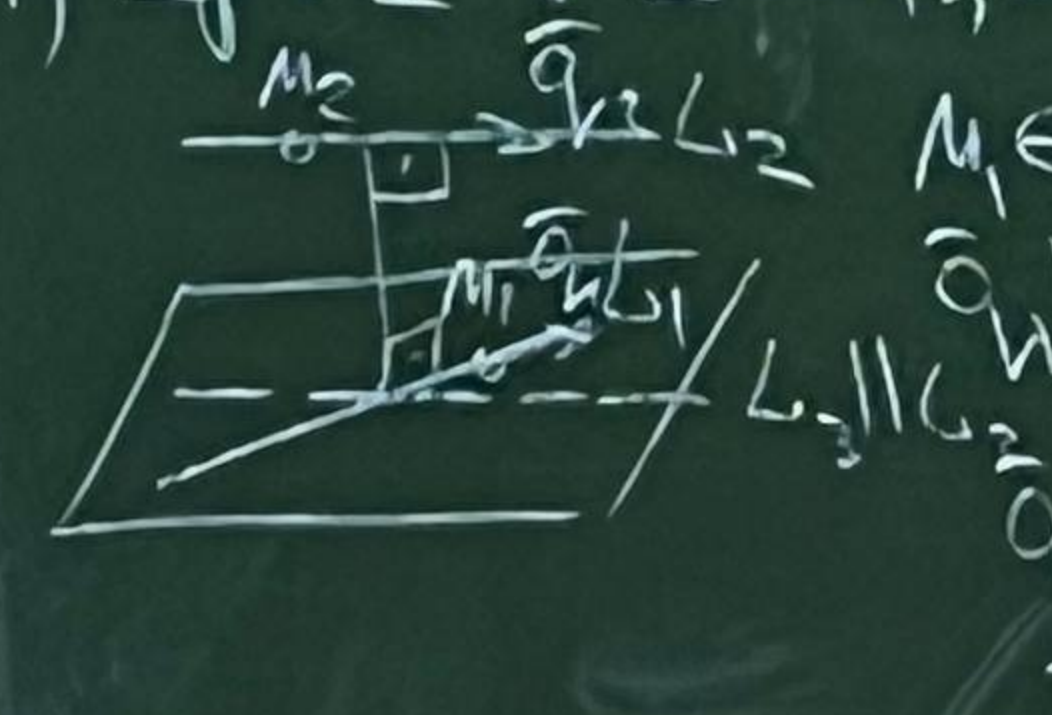
\includegraphics[scale=0.3]{images/2024-11-22/14.png}
\begin{align*}
    \text{Уравнение плоскости } P: P \in L_1, P \parallel L_2, L_1 \nparallel L_2 \\
    \begin{rcases}
        M_1 \in L_1 \Rightarrow M_1 \in P \\
        \overline{q}_1 \parallel L_1 \Rightarrow \overline{q}_1 \parallel P \\
        \overline{q}_2 \parallel L_2 \Rightarrow \overline{q}_2 \parallel P \\
        \overline{q}_1 \nparallel \overline{q}_2
    \end{rcases} \Rightarrow 
    \text{компланарное уравнение плоскости } P 
\end{align*}


\subsection{Пример}
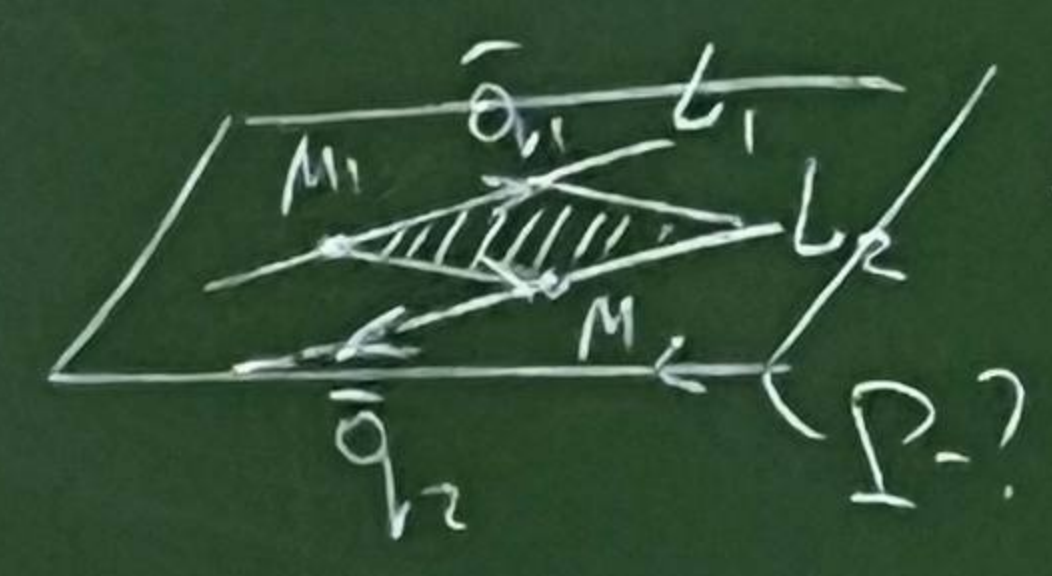
\includegraphics[scale=0.3]{images/2024-11-22/15.png}
\begin{align*}
    \text{Уравнение плоскости } P:
    \begin{rcases}
        M_1 \in P \\
        \overline{M_1 M_2} \parallel P \\
        \overline{q}_1 \parallel P \\
        \overline{M_1 M_2} \nparallel \overline{q}_1
    \end{rcases} \Rightarrow
    \text{компланарное уравнение плоскости P}
\end{align*}




%--------------------------------------------------
\newpage
\part{Нелинейные геометрические объекты на плоскости и в пространстве}

\section{Кривые 2-го порядка на $Oxy$}

\subsection{Определение | Кривая 2-го порядка}
Кривой второго порядка системы координат $Oxy$ называется геометрическое место точек $M(x, y) \in Oxy$:
\[
    \underbrace{\underbrace{Ax^2 + 2Bxy + Cy^2}_{\text{квадратичная форма}} + \underbrace{Dx + Ey + F}_{\text{линейная форма}} = 0}_{\text{общее уравнение кривой 2-го порядка}}
\]


\subsection{Типы}
\subsubsection{Эллипс}
Геометрическое место точек $M(x, y)$, сумма расстояний, каждое из которых до двух заданных фокусов ($F_1$ и $F_2$),
находящиеся на расстоянии $2c > 0$ является постоянной величиной равной $2a > 2c$:
\[
    \forall M(x, y) \in \text{ Эллипс }:~ MF_1 + MF_2 = 2a > 2c = F_1F_2
\]
(рисунок)
\begin{gather*}
    \text{Пусть } Oxy:~ F_1 \in Ox, F_2 \in Ox, OF_1 = OF_2 \\
    \Delta MEF_1:~ MF_1 = \sqrt{(x + c)^2 + y^2} ~~~~~
    \Delta MEF_2:~ MF_2 = \sqrt{(x - c)^2 + y^2}
\end{gather*}
\paragraph{Уравнение Эллипса} 
\[
    \sqrt{(x + c)^2 + y^2} + \sqrt{(x - c)^2 + y^2} = 2a, a > c > 0
\]
\paragraph{Иррациональное уравнение Эллипса}
\[
    \frac{x^2}{a^2} + \frac{y^2}{b^2} = 1, b = \sqrt{a^2 - c^2} > 0
\]
Выше каноническое уравнение Эллипса с полуосями $a, b > 0$, где
$b < a$: $a$ --- бОльшая полуось, $b$ --- меньшая полуось



\section{Поверхности 2-го порядка в $Oxyz$}
\subsection{Определение | Поверхность 2-го порядка}
Поверхностью второго порядка в системе координат $Oxyz$ называется \\ 
геометрическое место точек $M(x, y, z) \in Oxyz$:
\[
    Ax^2 + By^2 + Cz^2 + 2Dxy + 2Exz + 2Fyz + 2Gx + 2Hy + 2Jz + K = 0
\]
 

\subsection{Канонические уравнения}
Их исследование производится методом сечений плоскостями, параллельным координатным осям:
\[
    P_1 \parallel Oxy: z = d_1 ~~~~~
    P_2 \parallel Oyz: x = d_2 ~~~~~
    P_3 \parallel Oxz: y = d_3
\]

\subsubsection{Эллипсоид}
\[
    \frac{x^2}{a^2} + \frac{y^2}{b^2} + \frac{z^2}{c^2} = 1
\]
\textit{(изображения в планшете)}

\subsubsection{Мнимый эллипсоид}
\[
    \frac{x^2}{a^2} + \frac{y^2}{b^2} + \frac{z^2}{c^2} = -1
\]

\subsubsection{Однополосный гиперболоид}
\[
    \frac{x^2}{a^2} + \frac{y^2}{b^2} - \frac{z^2}{c^2} = 1
\]
\textit{(изображения в планшете)}

\subsubsection{Двухполосных гиперболоид}
\[
    \frac{x^2}{a^2} + \frac{y^2}{b^2} - \frac{z^2}{c^2} = -1
\]
\textit{(изображения в планшете)}

\subsubsection{Мнимый конус (точка)}
\[
    \frac{x^2}{a^2} + \frac{y^2}{b^2} + \frac{z^2}{c^2} = 0
\]

\subsubsection{Конус}
\[
    \frac{x^2}{a^2} + \frac{y^2}{b^2} - \frac{z^2}{c^2} = 0
\]
\textit{(изображения в планшете)}

\subsubsection{Эллиптический параболоид}
\[
    \frac{x^2}{a^2} + \frac{y^2}{b^2} = 2z
\]
\textit{(изображения в планшете)}

\subsubsection{Гиперболический параболоид}
\[
    \frac{x^2}{a^2} - \frac{y^2}{b^2} = 2z
\]
\textit{(изображения в планшете)}

\subsubsection{Эллиптический цилиндр}
\[
    \frac{x^2}{a^2} + \frac{y^2}{b^2} = 1
\]
\textit{(изображения в планшете)}

\subsubsection{Мнимый эллиптический цилиндр}
\[
    \frac{x^2}{a^2} + \frac{y^2}{b^2} = -1
\]

\subsubsection{Гиперболический цилиндр}
\[
    \frac{x^2}{a^2} - \frac{y^2}{b^2} = 1
\]
\textit{(изображения в планшете)}

\subsubsection{Пара мнимых пересекающихся плоскостей}
\[
    \frac{x^2}{a^2} + \frac{y^2}{b^2} = 0 ~~~~~ \text{ прямая, совпадающая с } Oz
\]

\subsubsection{Пара пересекающихся плоскостей}
\[
    \frac{x^2}{a^2} - \frac{y^2}{b^2} = 0
\]
\textit{(изображения в планшете)}

\subsubsection{Параболический цилиндр}
\[
    y^2 = 2px
\]
\textit{(изображения в планшете)}

\subsubsection{Пара мнимых параллельных плоскостей}
\[
    y^2 + b^2 = 0
\]

\subsubsection{Пара параллельных плоскостей}
\[
    y^2 - b^2 = 0
\]
\textit{(изображения в планшете)}

\subsubsection{Пара совпадающих плоскостей}
\[
    y^2 = 0
\]
\textit{(изображения в планшете)}



\end{document}
